\documentclass[a4paper, 12pt]{article}

\usepackage{fontawesome,wasysym, caption}
\usepackage{decorule,graphics, graphicx,subcaption}
\usepackage{float, amsmath}
\usepackage{geometry}


%opening
\title{Best practises for my Bachelor}
\author{me \faMoonO}
\geometry{top=2.5cm, bottom=3.5cm, left=2.5cm, right=2.5cm}

\begin{document}

\maketitle
\setlength{\parindent}{0em}
\setlength{\parskip}{0.5em}
\renewcommand{\baselinestretch}{1}

\section{Examples}

\faChevronCircleRight\hspace{0.5cm} Einfügen ein Bild\\
\textbf{Specifier:}\\ h: Place the float here, i.e., approximately at the same 
point it occurs in the source text (however, not exactly at the spot).\\ t: 
Position at the top of the page.\\ b: Position at the bottom of the page.\\ 
p: Put on a special page for floats only.\\ !: 	Override internal parameters 
LATEX uses for determining "good" float positions.\\ H: Places the float at 
precisely the location in the LATEX code. Requires the float package 
(\verb|usepackage{float}|). This is somewhat equivalent to h!, though some 
errors may arise if you have too many consecutive floats with [H].
\begin{verbatim}
	\begin{figure}[specifier]
	\centering
	\label{fig: sun}
	\includegraphics[width=7cm]{sun.jpg}
	\caption[Sunset]{An awesome sunset.}
	\end{figure}
\end{verbatim}
\begin{figure}[ht]
	\centering
	\label{fig: sun}
	\includegraphics[width=7cm]{images/sun.jpg}
	\caption[Sunset]{An awesome sunset.}
\end{figure}
\pagebreak
\faChevronCircleRight\hspace{0.5cm} Einfügen eine Gleichung
\begin{itemize}
	\item Möglichkeit 1: ohne Nummerierung
	\begin{verbatim}
	\[a^2+b=c/4\]
	\end{verbatim}
	\[a^2+b=c/4\]
	\item Möglichkeit 2: mit Nummerierung
	\begin{verbatim}
			\begin{split}
			&5^2+9^2=a^2\\
			&a=\sqrt{5^2+9^2}
			\end{split}
	\end{verbatim}
\begin{equation}
	\begin{split}
		% sign & used for allignment, split used to make some lines in one equation
	&5^2+9^2=a^2\\
	&a=\sqrt{5^2+9^2}
	\end{split}
\end{equation}
\end{itemize}

%	\triangle ABC \space ist ein rechteckiges Dreieck -> \angle BCA = 
%90^{\circ}\\
%\sqrt[3]{5^2+13^2}

%a \cdot f = 5\\
%z \times (m/2)=d^2
\faChevronCircleRight
\hspace{0.5cm}Ein bisschen Mathe
\begin{figure}[ht]
	\centering
	\captionsetup{justification=centering}
	\label{fig: formula}
	\includegraphics[width=6cm]{LaTeX_Formula.png}
	\caption[Formeln]{Standarten Mathe Formeln.}
\end{figure}
\pagebreak

\faChevronCircleRight
\hspace{0.5cm}Schriftarten
\begin{figure}[H]
	\centering
	\captionsetup{justification=centering}
	\label{fig: fonts}
	\includegraphics[width=6.5cm]{LaTeX_fonts.png}
	\caption[Formeln]{LaTeX Anweisungen, die die Schriftart ändern.}
\end{figure}



\end{document}
